\documentclass[twocolumn]{article}
\usepackage[margin=0.7in]{geometry} 
\usepackage{graphicx, wrapfig}
\usepackage{palatino}
\usepackage{subcaption}
\usepackage{multirow}
\usepackage{booktabs}
\begin{document}
\title{\vspace{-4ex}HW2: POS Tagging with HMM and CRF}
\author{Rahul Huilgol (rrh2226)}
\date{}
\maketitle
\vspace{-5mm}
\section{Introduction}
A good part of speech tagger considers globally what labelling of tags would give the most probable assignment. Hidden Markov Model (HMM) and Conditional Random Field (CRF) are probabilistic sequence labelling algorithms. 

HMM works on the idea that there are hidden states which form a finite state machine whose transitions are probabilistic and have a Markov property. Each of these states have particular distributions for producing observations. It models the joint distribution of labels and observations, and thus is a generative model. HMM can produce the most likely state sequence underlying an observation. In our case, an observation is a sentence. HMM can find the most likely underlying POS tags. They are trained using dynamic programming, and don't require multiple iterations.

CRF is a discriminative model, an undirected probabilistic graphical model, that is trained to maximize the performance of classification by modelling the conditional distribution of POS tags given the sequence. It models the conditional distribution similar to how multinomial logistic regression works. The parameters are learnt by Maximum likelihood projection using an optimization method like L-BFGS. 
\section{Experimental setup}
Datasets used for comparing  HMM and CRF at the task of POS tagging in this homework are ATIS and WSJ. All results for ATIS dataset are shown by averaging over 10 runs, each of which has randomized split of data in the form of 80-20 for training and test respectively. Since the WSJ dataset is very large and using the whole would take lot of time, few sections only have been used in this homework. Unless otherwise mentioned, results for WSJ here use first section for training and second section for testing.
\section{Results}
\begin{table}[h]
\centering
  \caption{HMM vs CRF vs CRF* (CRF* refers to CRF with extra features for each word)}
  \label{tab:first}
\begin{tabular}{@{}llllll@{}}
\toprule
\textbf{Model} & \textbf{Data} & \multicolumn{3}{c}{\textbf{Accuracy}}               & \textbf{Time} \\ \midrule
               &               & \textbf{Training} & \textbf{Testing} & \textbf{OOV} &               \\ \midrule
HMM            & ATIS          & 0.890             & 0.865            & 0.219        & 5      \\ \midrule
CRF            & ATIS          & 0.999             & 0.929            & 0.246        & 99      \\ \midrule
CRF*           & ATIS          & 0.999             & 0.933            & 0.332        & 90      \\ \midrule
HMM            & WSJ           & 0.862             & 0.785            & 0.379        & 76      \\ \midrule
CRF            & WSJ           & 0.986             & 0.794            & 0.476        & 6817      \\ \midrule
CRF*           & WSJ           & 0.991             & 0.843            & 0.640       &  6491      \\ \bottomrule
\end{tabular}
\end{table}
\begin{table}[h]    
        \centering
        \caption{Importance of each feature, tests on WSJ\\}
        \label{tab:second}
\begin{tabular}{@{}lllll@{}}
\toprule
\textbf{Extra Feature} & \multicolumn{3}{c}{\textbf{Accuracy}}               & \textbf{Time} \\ \midrule
                       & \textbf{Training} & \textbf{Testing} & \textbf{OOV} &               \\ \midrule
Caps                   & 0.989             & 0.823            & 0.562        & 7004       \\ \midrule
NumeroAlpha            & 0.986             & 0.798            & 0.492        & 7293       \\ \midrule
Hyphen                 & 0.987             & 0.790            & 0.477        & 6230       \\ \midrule
Suffix Few      & 0.986             & 0.808            & 0.526        & 4984       \\ \midrule
Suffix Many       & 0.988             & 0.828            & 0.599        & 7708       \\ \midrule
Prefix                 & 0.986             & 0.794            & 0.476        & 5438       \\ \midrule
Prefix \& Suffix      & 0.986              & 0.808            & 0.524        & 6745        \\ \bottomrule
\end{tabular}
\end{table}
\begin{table}[h]    
\centering
\begin{tabular}{@{}lllllll@{}}
\toprule
\textbf{Model} & \textbf{Data} & \multicolumn{3}{c}{\textbf{Accuracy}}               & \textbf{Time} \\ \midrule
               &  Sections     & \textbf{Training} & \textbf{Testing} & \textbf{OOV} &               \\ \midrule
HMM            & 1                     & 0.862             & 0.785            & 0.379        & 80       \\ \midrule
HMM            & 2                     & 0.887             & 0.833            & 0.396        & 233       \\ \midrule
CRF            & 1                     & 0.986             & 0.794            & 0.476        & 3350       \\ \midrule
CRF*           & 1                     & 0.991             & 0.843          & 0.640        & 6491   \\ \midrule
CRF            & 2                     & 0.994             & 0.842            & 0.500        & 20081      \\ \midrule
CRF*           & 2                     & 0.994             & 0.895            & 0.737        & 20084     \\ \bottomrule
\end{tabular}
\caption{Training on larger WSJ data}
\label{largedata}
\end{table}
Table \ref{tab:first} provides a comparision of HMM and CRF on ATIS and WSJ. Here when modelling WSJ dataset, the first section was used for training and second section for testing. We see here that for ATIS, CRF beats HMM significantly on test accuracy. When we consider the larger data, one section of WSJ, there is not much difference. CRF beats HMM just by 1\%. The reason can be attributed to the fact that HMM is generative and CRF is discriminative. A discriminative model works much better for small data, because it has to only focus on learning the conditional distribution. For larger data, this advantage reduces. HMM performs better. 

OOV accuracy is defined as the number of Out of vocabulary words that the model could predict the correct POS tag, where Out of vocabulary means words not seen during training. This is a much more difficult task, so the OOV accuracy is much lower than the overall accuracy. CRF performed better than HMM at OOV, and has almost 10\% higher OOV accuracy on WSJ and some increase on the ATIS as well. This can be attributed to the fact that CRF models the tries to estimate conditional probability directly, and draws from the information it learnt during training to predict POS tag for a new word. HMM on the other hand models the joint distribution of tags and words. Because HMM does not know about these OOV words, it performs badly on it. 

CRF consistently shows a really high accuracy (around 99\%) on the training set. This is a sign that it is overfitting the training data. HMM on the other hand does not show this effect with training accuracies in the range of 85-90\%. This could be because a HMM tries to fit a distribution to the training data, that is it tries to find out a probability distribution which generates it. It does not try to fit every data point into the model it is building. A discriminative classifier is free in the choice of the decision function it learns and can fit all samples. So the discriminative models are more likely to overfit.


When we compare the times taken by HMM and CRF, we see a drastic difference. HMM only takes a fraction of the time to train. Like Table \ref{tab:first} shows, on one section of WSJ, HMM took around a minute (76sec) and CRF took 1 hour and 53 minutes(6800sec). This is almost 100 times more. This is because a HMM only needs to estimate frequency counts to build its model. CRF on the other hand needs to solve a difficult optimization problem. This is done by maximum likelihood estimation and needs many iterations to converge. When looking at the times, there might be slight discrepancies because all the jobs were run using the UTCS Condor cluster, and different capacities and workloads of processors greatly affected the run times.


CRF* is the CRF model which also considers additional orthographic features provided to it. Features provided include if first character is capitalized, first character is number, word contains hyphen, words contains a suffix and word contains a prefix. These features should help OOV accuracy for CRF  because the model can use such features from test tokens and predict POS tag using the information it learned about such features from training. It has a significant effect as Tables \ref{tab:first} and \ref{largedat} show. Overall test accuracy for CRF* is higher than CRF by 5\% on WSJ. The OOV accuracy for CRF* is a whopping 17\% higher than CRF. A HMM model can not incorporate such additional features. Overall, when we compare HMM with CRF*, there is a tremendous difference in accuracies. I did not notice much effect on the run time of the model, it almost stayed the same. It is hard to say if there was any small effect on the time, because of the large variance in timings as discussed above.

% \subsection{Comparing importance of the orthographic features introduced}
I also compared how important each of the orthographic features mentioned above were. To do this I only introduced one type of feature and trained the CRF* model. Results for WSJ data are shown in Table \ref{tab:second}. \textit{Suffix Few} refers to a short list of 39 suffixes and \textit{Suffix Many} refers to a longer list of 123 suffixes. Number of prefixes considered for \textit{Prefix} are 42. Please note that the CRF* in Table \ref{tab:first} uses all the orthographic features. We see here that whether a word starts with a digit or contains a hyphen or starts with a prefix does not seem to show a significant change in accuracies. This indicates that they are not probably not very important for CRF tagging. The longer list of suffixes is not surpisingly better than the shorter list. Capitalization also showed a strong effect, which makes sense because whether a word starts with a capital letter has a strong relationship with whether it is a proper noun.


Table \ref{largedata} shows the accuracies with more sections of WSJ data. CRF on two sections took a very long time (5.5 hrs). Both models showed considerably improved accuracies. CRF* with just two sections achieved  a surprising 74\% OOV accuracy. This I found to be a testament to why CRF's are considered to be almost state of the art. The drastically shorter time means HMM also are useful when there is not much time. While the overall accuracy of HMM are not too bad, they are particularly bad on OOV accuracy.


HMM's do not have to iterate and converge while training. So their accuracies stayed almost the same irrespective of how many iterations it took for the given HMMSimpleTagger to run. But Fig \ref{fig:crf} shows how accuracies change with increased number of iterations.
\begin{figure}
\begin{center}
    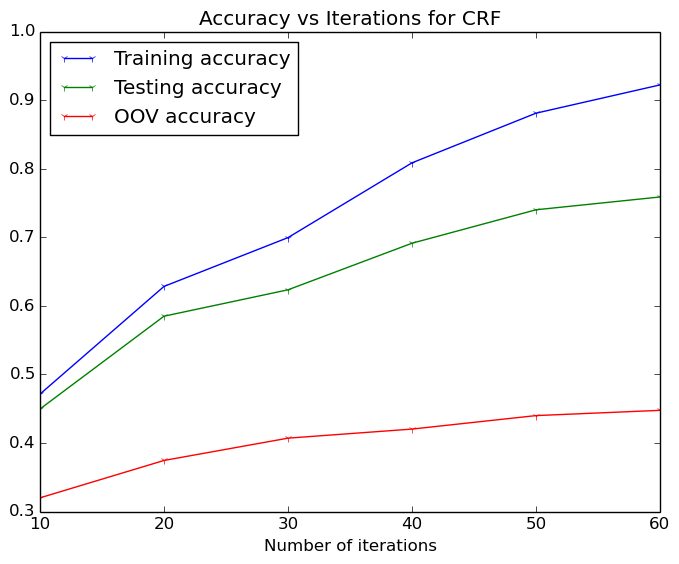
\includegraphics[width=0.45\textwidth]{crf_iters.png}
    \caption{CRF}
    \label{fig:crf}
    \end{center}
\end{figure}
\vspace{-3mm}
\section{Conclusion}
\vspace{-3mm}
HMMs take a fraction of the time taken by CRFs. But CRFs are significantly better than HMMs if given enough time to train. Adding orthographic features is immensely helpful, and this gives CRF a major advantage.
\end{document}
